\section{Planification du projet}
\label{sec:orga}

	Les différents délivrables du projet 4INFO imposent une gestion de projet suivant un modèle de cycle en V. Cependant, nous sommes libres d'adapter nos propres méthodes de développement 

	Ici, nous avons de nombreuses fonctionnalités que nous allons être amené à réaliser. Il est donc nécessaire de penser à une bonne méthode de gestion lors du développement. Cela nous permettra de gérer au mieux le temps qui nous est imparti en prenant en compte les ressources que nous avons à disposition notamment humaines. D'un côté, il est nécessaire d'évaluer l'importance de chaque fonctionnalité, définie bien précisément, et de l'autre, la partie la plus complexe, il nous faut estimer la durée pour réaliser chaque tâche.

	En respectant un modèle de cycle en V, nous nous retrouverions donc à développer la plateforme, puis à effectuer différentes séries de tests avant de la délivrer. Le problème de cette méthode est que nous allons devoir faire une sélection de fonctionnalités à développer, s'y tenir, et un livrable ne sera fournit qu'à la fin. Entre autre, nous ne pourrons avoir un retour sur l'application que lorsque le développement sera fini. Il sera impossible d'inférer sur les fonctionnalités puisqu'il n'y aura aucun retour durant le temps de développement. 

	C'est pourquoi nous pensons planifier le développement de l'application en se basant sur les méthodes agiles. Nous aurons donc une liste de fonctionnalités, triée suivant leur importance et leur difficulté à être développées. En considérant les ressources mises à disposition, nous délivrerons et effectuerons en continue des tests pour chacune des fonctionnalités. Ainsi il sera possible de présenter l'avancement au milieu du projet à nos encadrants, et il serait possible de redéfinir certaines priorité pour les fonctionnalités restantes, ou en rajouter par la suite si nous prenons de l'avance sur le développement. Si celles-ci se trouvent être plus intéressantes (ou plus faciles), nous pourrions nous retrouver à les développer en priorité par rapport à des fonctionnalités définies avant. Enfin, cela permet à un instant T d'avoir un produit fonctionnel.

	En faisant une liste non exhaustive de tâches globales (on ne détaille pas encore toutes les sous-tâches de développement qu'une tâche implique, et les tests sont inclus dans le temps de la tâche), et en les ordonnant de manière à obtenir une plateforme qui contiendra au fur et à mesure de plus en plus de fonctionnalités en partant des plus importantes; on arrive à ce schéma de planification.

	\begin{figure}[H]
        \centering
        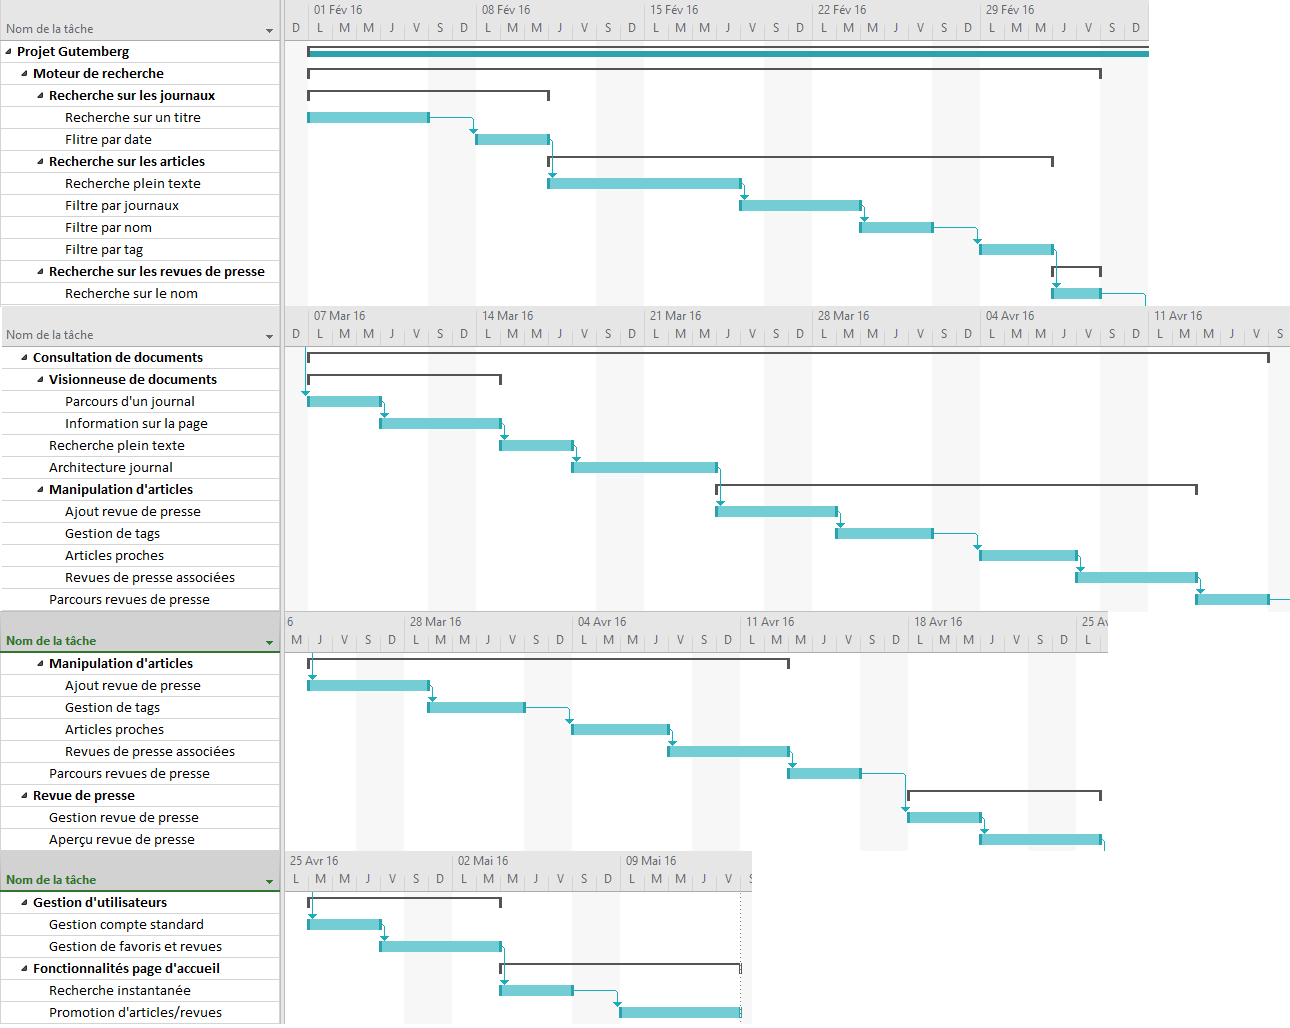
\includegraphics[width=1.3\textwidth, angle=90]{figures/plan.png}
            \caption{Plannification}
            \label{fig:plan_recherche}
    \end{figure}